\documentclass[../DS08.tex]{subfiles}%
\graphicspath{{./figures/}}%

% \subimport{/home/nora/Documents/Enseignement/Prepa/bpep/exercices/TD/autour_E-pH_du_chlore/}{sujet.tex}%

\usetikzlibrary{circuits.ee.IEC}
\usetikzlibrary{babel}

\begin{document}%
\prblm[64]{Exploitation du diagramme $E-\pH$ du chlore\ifcorrige{~\small\textit{(D'après
			Centrale TSI 2018)}}}%

\subsection{Diagramme du chlore}%

La figure~\ref{fig:E-pHCl} donne le diagramme potentiel$-\mathrm{pH}$ de l'élément
chlore. Les espèces considérées, qui sont toutes en solution, sont
$\ce{Cl2_(aq)}$, $\ce{Cl^-_{(aq)}}$, $\ce{ HClO_{(aq)}}$ et $\ce{ClO^-_{(aq)}}$. La
concentration de tracé est $c = \SI{1,0e-1}{ \mol \per\liter}$. Les
frontières entre deux espèces ont été calculées en traduisant
l'égalité des \emph{concentrations molaires en élément} chlore de
chaque espèce sur la frontière, la somme de ces concentrations étant
égale à $c$.

\begin{figure}[h]
	\centering
	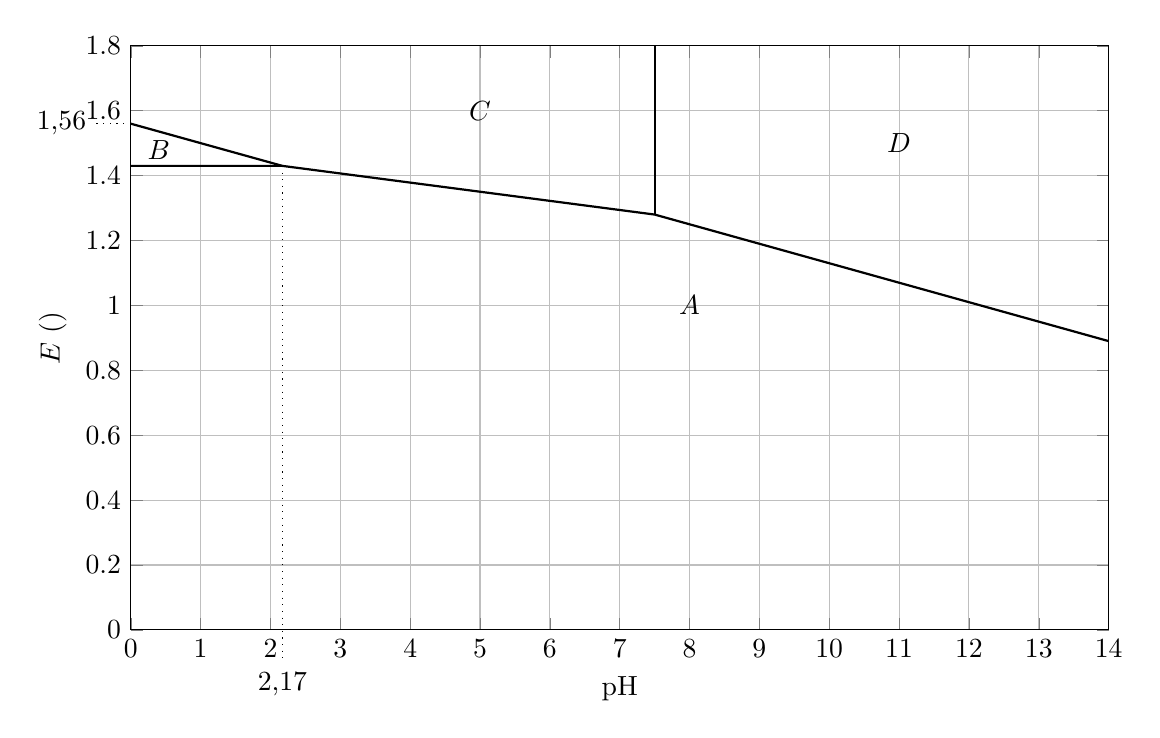
\begin{tikzpicture}%
		%\usetikzlibrary{svg.path}%
		\begin{axis}[
				clip=false,
				width=140mm, height=90mm,
				xmin=0, xmax=14,
				xlabel=$\mathrm{pH}$,
				ymin=0, ymax=1.8,
				ylabel=$E$ (\si{\volt}),
				grid=both,
			]
			\addplot [thick] coordinates{(0, 1.43) (2.17, 1.43)  (7.5, 1.28) (14, 0.89)};
			\addplot [thick] coordinates{(0, 1.56)  (2.17, 1.43)};
			\addplot [thick] coordinates{(7.5, 1.28)  (7.5, 1.8)};

			\addplot [dotted] coordinates{(2.17, 1.43) (2.17,-.1)} node [below] {2,17};
			\addplot [dotted] coordinates{(0, 1.56)  (-.5,1.56)} node [left] {1,56};
			%    
			\addplot [dotted] coordinates{(8, 1)} node {$A$};
			\addplot [dotted] coordinates{(0.4, 1.48)} node {$B$};
			\addplot [dotted] coordinates{(5, 1.6)} node {$C$};
			\addplot [dotted] coordinates{(11, 1.5)} node {$D$};
		\end{axis}%
	\end{tikzpicture}%
	\caption{Diagramme E-pH du chlore}%
	\label{fig:E-pHCl}%
\end{figure}%


\QR{%
Justifier que les espèces $A$, $B$, $C$ et $D$ sont
respectivement $\ce{Cl^-_{(aq)}}$, $\ce{Cl_{2\,(aq)}}$, $\ce{HClO_{(aq)}}$ et
$\ce{ClO^-_{(aq)}}$.
}{%
On calcule le degré d’oxydation de l’atome de chlore dans les différents édifices chimiques, ainsi $no(\ce{Cl / Cl-}) = -I$, $no(\ce{Cl / Cl2}) = 0$, $no(\ce{Cl / HClO}) = +I$ et $no(\ce{Cl / ClO^-}) = +I$. Ainsi \ce{Cl-} ayant le plus faible degré d’oxydation doit se situer dans le domaine de potentiel le plus faible c’est à dire $A$. On remarque ensuite une frontière horizontale entre $A$ et $B$, ce qui caractérise un échange d’électrons uniquement, donc $B :\ce{Cl2}$. Ce qui est confirmé par le fait que ce soit le seul élément avec un nombre d'oxydation intermédiaire (0), et pouvant ainsi avoir un niveau d'oxydation plus grand que celui de $A$ et plus faible que celui de $C$. Enfin les deux dernières espèces ont le même degré d’oxydation, le plus grand, donc $+I$, l’espèce acide étant $C$ et l’espèce basique étant $D$. On en déduit donc que $C :\ce{HClO}$ et $D :\ce{ClO-}$.
}%


\QR{%
	Déterminer le $pK_a$ du couple $\ce{HClO / ClO^-}$.
}{%
	Par définition,  $K_a = \frac{[\ce{ClO-}][\ce{H+}]}{[\ce{HClO}]}$. Or cette  équilibre est atteint sur la frontière verticale, il y a donc alors égalité des concentrations d’après l’énoncé,  et ainsi $\mathrm{pK_a} = \mathrm{pH}$. Donc par lecture graphique $\boxed{\mathrm{pK_a} = \num{7,5}}$
}%


\QR{%
Déterminer le potentiel standard du couple $B/A$.
}{%
La demi  équation rédox du couple \ce{B/A} est \ce{Cl2 + 2 e- = 2 Cl-}, ainsi l’équation de la frontière est donnée par \[E = E^\circ  + \frac{\num{0, 06}}{2}\log \frac{[\ce{Cl2}]}{[\ce{Cl^-}]^2 }\]

On nous signale qu’il y a  égalité des concentrations en  éléments sur la frontière, donc $2[\ce{Cl2}] = [\ce{Cl^-}]$, et comme $2[\ce{Cl2}] + [\ce{Cl^-}] = c$, nous avons que $[\ce{Cl2}] = c/4$ et $[\ce{Cl^-}] = c/2$. Finalement $E = E^\circ  - \num{0, 03} \log c$.

Pour déterminer $E$ on peut utiliser les informations sur la frontière entre $B$ et $C$:
\[
	\ce{2 HClO + 2 H+ + 2 e^- = Cl2 + 2 H2O},
\]
ainsi la pente est de \SI{0,06}{\volt\per pH}, et ainsi $E = \SI{1, 56}{\volt} - \SI{0,06}{\volt\per pH} \cdot \SI{2, 17}{pH} = \SI{1, 43}{\volt}$. En conclusion, $\boxed{E^\circ  = E+\num{0, 03} \log c=\SI{1, 40}{ V}}$.
}%


\QR{%
	Écrire la demi-équation redox entre les espèces $A$ et $C$.
}{%
	\ce{HClO + H^+ + 2 e^- = Cl^- + H2O}%
}%


\QR{%
	Déterminer la pente de la frontière $C/A$ et en effectuer
	la vérification graphique.
}{%
	À partir de la demi-équation  électronique on en déduit que la pente est de \SI{-0, 03}{\volt\per pH}. En prolongeant la frontière, on remarque qu’elle passe par les points $(2, 17 ;1,43)$ et $(10,5 ;1,2)$, ce qui confirme une pente de \SI{-0, 03}{\volt\per pH}%
}%


\QR{%
	Déterminer le potentiel standard du couple $C/A$.
}{%
	La formule de \textsc{Nernst} pour ce couple donne $E = E^\circ  + \num{0, 03} \log \frac{[\ce{HClO}][\ce{H^+}]}{[\ce{Cl^-}]}$. Or il y a  égalité des concentrations sur la frontière, ainsi $E = E^\circ  - \SI{0, 03}{pH}$. En $\mathrm{pH} = \num{2, 17}$, $ E = \SI{1, 43}{\volt}$, ainsi $E^\circ  = \SI{1, 43}{V} + \SI{0, 03}{\volt\per pH} \cdot \SI{2.17}{pH} = \SI{1, 50}{ V}$
}%


\subsection{Diagramme de l'eau}%

\enonce{
	On considère les espèces $\ce{H2O}$, $\ce{O2_{(g)}}$ et $\ce{
			H2_{(g)}}$. La pression de tracé est fixée à \SI{1}{ \bar} et la
	concentration de tracé à \SI{1,0}{\mol\per\liter}.}%

\QR{%
	Déterminer l'équation de la frontière $\ce{O2_{(g)} / H2O}$.
}{%
	\ce{O2 + 4 H^+ + 4 e^- = 2 H2O}, d’où $E = E^\circ  - \SI{0, 06}{pH} = \SI{1, 23}{V} - \num{0, 06}\cdot pH\si{V}$ avec les informations de l’énoncé (pression de \SI{1}{bar}).
}%


\QR{%
	Déterminer l'équation de la frontière $\ce{H_2O / H2_{(g)}}$.
}{%
	\ce{H2O + 2 H^+ + 2 e^- = H2 + H2O}, d’où $E = E^\circ  - \SI{0, 06}{\volt\per pH}\cdot pH = -\SI{0, 06}{\volt\per pH}\cdot pH$
}%


\QR{%
	Tracer succinctement sur votre copie l'allure du diagramme potentiel$-\mathrm{pH}$ de l'eau superposé à celui du chlore aqueux. Quels commentaires pouvez-vous
	formuler ?
}{%
	les lignes de séparation des domaines de l'eau partent à pH=0 à 0 et \SI{1,23}{V} respectivement, avec une pente de \SI{-,06}{\volt\per pH}, elles sont intégralement en dessous de tous les autres segments du diagramme E-pH.
	En superposant ces deux diagrammes, nous remarquons que seul \ce{Cl^-} peut coexister dans l’eau car toutes les autres espèces ont des domaines disjoints avec celui de l’eau.
}%


\subsection{Étude de la cellule d'électrolyse}%
\begin{minipage}{.48\columnwidth}%
	\begin{center}%
		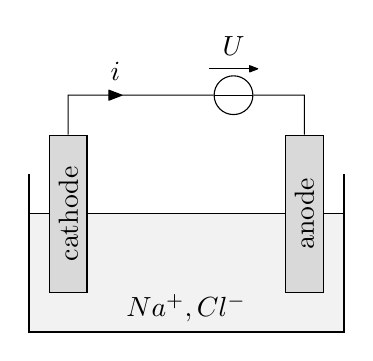
\begin{tikzpicture}[circuit ee IEC]
			%\usetikzlibrary{svg.path}%
			\fill [black!5] (-2, 1.5) rectangle (2, 0);
			\draw [thick] (-2, 2) |- (2, 0) -- (2, 2);
			\draw (-2, 1.5) -- (2, 1.5);
			\node at (0, 0) [above] {$\ce{Na^+, Cl^-}$};
			\node (cathode) at (-1.5, 1.5) [rotate=90, draw, fill=black!15, minimum width=20mm] {cathode};
			\node (anode) at (1.5, 1.5) [rotate=90, draw, fill=black!15, minimum width=20mm] {anode};
			\draw
			(cathode.east) -- ++(0, 0.5) coordinate (C)
			to [current direction={pos=0.2, info=$i$},
					voltage source={pos=0.7, direction info={info=$U$}}] (C -| anode.east) -- (anode.east);
		\end{tikzpicture}%
		\captionof{figure}{L'électrolyseur}%
		\label{fig:électrolyseur}%
	\end{center}%
\end{minipage}%
\begin{minipage}{.5\columnwidth}%
	L'électrolyseur est constitué de deux électrodes en titane. Le schéma
	de principe est donné figure~\ref{fig:électrolyseur}. La tension $U$ et
	le courant $i$ sont des grandeurs positives. Lors de la mise sous
	tension de l'électrolyseur, on observe une production de $\ce{
			H2_{(g)}}$ et de $\ce{Cl2_{(aq)}}$. L'électrolyseur est placé en
	amont du système de filtrage de l'eau.
\end{minipage}%

\QR{%
	Écrire les demi-réactions électroniques des réactions se
	déroulant à l'anode et à la cathode.
}{%
	À l’anode il se produit une oxydation, ainsi il se produit du \ce{Cl2} selon la réaction \ce{2 Cl^- = Cl2 + 2 e^-}.

	À la cathode, il se produit une réduction, donc la formation de \ce{H2} selon la réaction \ce{2 H+ + 2 e^- = H2}%
}%


\enonce{
	L'eau d'une piscine est maintenue à un $\mathrm{pH}$ compris entre \num{7,0} et \num{7,4}.}%

\QR{%
Écrire l'équation modélisant la réaction chimique qui, à partir de $\ce{Cl2_{(aq)}}$ en solution aqueuse, forme $\ce{Cl^-_{(aq)}}$ et $\ce{ClO^-_{(aq)}}$.
}{%
On  écrit les deux demi-équations  électroniques qui interviennent ici :

\ce{Cl2 + 2 e^- = 2 Cl^-}%


\ce{Cl2 + 2 H2O = 2 ClO^- + 4 H^+ + 2 e^-}%

Ainsi en combinant ces deux demi-équations pour éliminer les  électrons  échangés, nous obtenons, après simplification:
\ce{ Cl2 + H2O = Cl^- + ClO^- + 2 H^+}%
}%


\QR{%
	Comment appelle-t-on ce type de réaction ?
}{%
	C'est une réaction de dismutation.
}%


\enonce{
	On envisage dans la suite une piscine de particulier de contenance
	$V_0 = \SI{150}{\cubic\meter}$.}%

\QR{%
	Avant la mise en fonctionnement de l'électrolyseur, l'eau
	de la piscine doit être salée avec une teneur en sel d'environ $c_s =
		\SI{5}{\gram\per\liter}$ (on prendra cette valeur pour les applications
	numériques). Quelle masse de sel le particulier doit-il acheter lors
	de la première mise en route du dispositif ?
}{%
	$m = c_s\cdot V_0 = \SI{5}{\gram\per\litre} \cdot \SI{150}{\cubic\meter} = \SI{750}{kg}$
}%

\enonce{
	Un fabriquant d'électrolyseurs de piscines annonce, pour un modèle
	adapté à un volume maximal de bassin de \SI{150}{\cubic\meter}, une
	production horaire maximale $\dot m_\text{max} = \SI{26}{\gram\per \hour}$
	de $\ce{Cl2}$. Pour ce modèle, $U = \SI{7,5}{\volt}$.}%

\QR{%
	Calculer la valeur de $i$ correspondant au fonctionnement
	maximal. On supposera le fonctionnement idéal.
}{%
	Cherchons la quantité de dichlore formée par seconde:
	\[
		n_{\ce{Cl2}} = \frac{m_{\text{max}}}{2 M_{\ce{Cl}}\times\SI{3600}{\second\per\hour}}%
	\]
	Or la formation à l’anode d’une mole de \ce{Cl2} s’accompagne de la libération de 2 moles d’électrons, ainsi $n_e = 2 n_{\ce{Cl2}}$.

	Finalement, $\boxed{i = e \mathcal N_a \frac{n_e}{\SI{1}{\second}} = \mathcal{F} \frac{m_{\text{max}}}{M_{\ce{Cl}}\times\SI{3600}{\second\per\hour}}
			= \SI{20}{ A}}$.
}%


\QR{%
	Calculer la puissance correspondant à une production
	horaire maximale. Commenter le résultat.
}{%
	$P = U I = \SI{150}{W}$,  ce qui n’est pas excessif, sauf s'il faut la faire tourner en continu…
}%

\end{document}%
